\documentclass[12pt]{article}

\usepackage[margin=1.0in]{geometry}
\usepackage{tabto}
\usepackage{amsmath}
\usepackage{framed}
\usepackage{graphicx}
\usepackage{listings}
\usepackage{color} %red, green, blue, yellow, cyan, magenta, black, white
\definecolor{mygreen}{RGB}{28,172,0} % color values Red, Green, Blue
\definecolor{mylilas}{RGB}{170,55,241}
\graphicspath{ {./} }

\newcommand*\lstinputpath[1]{\lstset{inputpath=#1}}



\begin{document}

\title{CS / MATH 4334 : Numerical Analysis\\Homework Assignment 4}
\author{Matthew McMillian\\mgm160130@utdallas.edu}
\maketitle

\section*{MatLab Problems}

\lstset{language=Matlab,%
    %basicstyle=\color{red},
    breaklines=true,%
    morekeywords={matlab2tikz},
    morekeywords=[2]{1}, keywordstyle=[2]{\color{black}},
    identifierstyle=\color{black},%
    showstringspaces=false,%without this there will be a symbol in the places where there is a space
    numbers=left,%
    numberstyle={\tiny \color{black}},% size of the numbers
    numbersep=9pt, % this defines how far the numbers are from the text
    emph=[1]{for,end,break},emphstyle=[1]\color{red}, %some words to emphasise
    %emph=[2]{word1,word2}, emphstyle=[2]{style},    
}

\pagebreak

	\begin{enumerate}
	
	\item[] Problem 1 : p1.m \noindent\rule{\textwidth}{1.0pt} \\
	\lstinputlisting{p1.m}
	
	\item[] Problem 1 : p1chev.m \noindent\rule{\textwidth}{1.0pt} \\
	\lstinputlisting{p1chev.m}	
	
	\pagebreak	
	
	$>>$ p1.m
	\begin{framed}
	abserr =\\

     2.142188221906679e-01\\


	abserr =\\

     1.894862537027103e+03\\

	\end{framed}
	
    $>>$ p1chev.m
	\begin{framed}
	
	abserr =\\

     2.872137290339052e-01\\


	abserr =\\

     9.477703742070265e-02\\
     
     You can compute the error bounds of both (a) and (b) since you have access to the initial function. If you only had data points, you could not compute the theoretical error.
	\end{framed}
	
		\begin{center}
			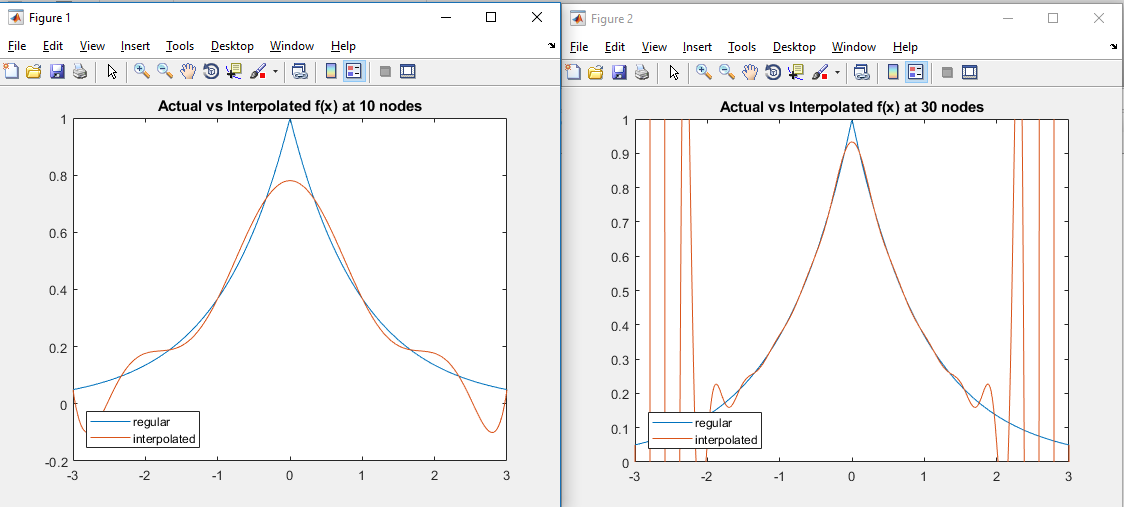
\includegraphics[scale=0.55]{hwg1}
		\end{center} 
		
			\begin{center}
			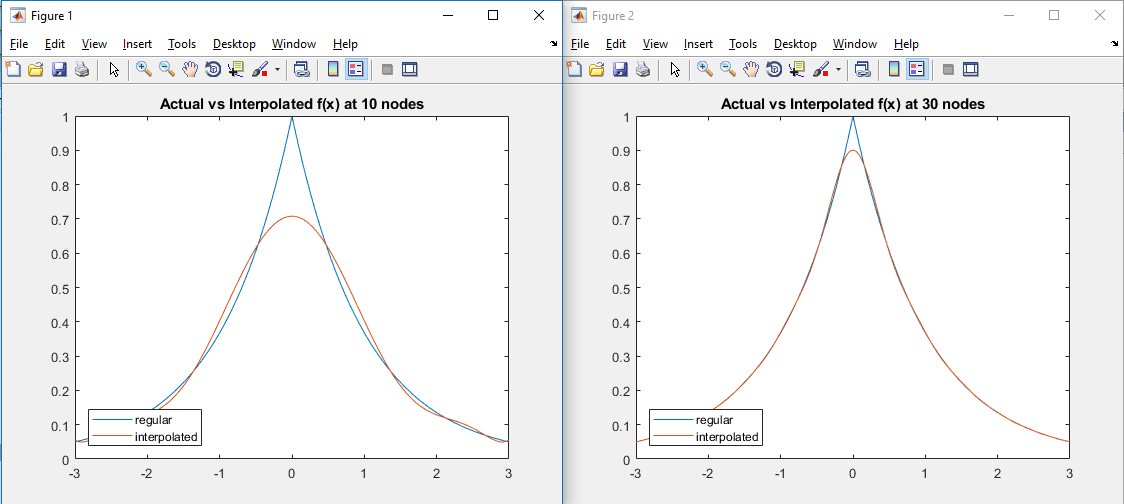
\includegraphics[scale=0.55]{hwg2}
		\end{center} 
	
	\end{enumerate}
	
\pagebreak	
	
	\begin{enumerate}
	
	\item[] Problem 2 : quadspline.m \noindent\rule{\textwidth}{1.0pt} \\
	\lstinputlisting{quadspline.m}	
	
	\item[] Problem 2 : cosine.m \noindent\rule{\textwidth}{1.0pt} \\
	\lstinputlisting{cosine.m}	
	
	\pagebreak	
	
	$>>$ quadspline.m
	\begin{framed}
	Example System for n=5: \\
	1 0 0 0-----b1------v1\\
	1 1 0 0-----b2------2/delta * (y3-y2) - v1\\
	0 1 1 0--*--b3--=---2/delta * (y4-y3) - 2/delta * (y3-y2)\\
	0 0 1 1-----b4------2/delta * (y5-y4) - 2/delta * (y4-y3)\\
	
	Det(A) = 1\\

ans =\\

     2.409905359662697e-01\\


ans =\\

     8.623460672974910e-01\\
	\end{framed}
	
	\begin{center}
			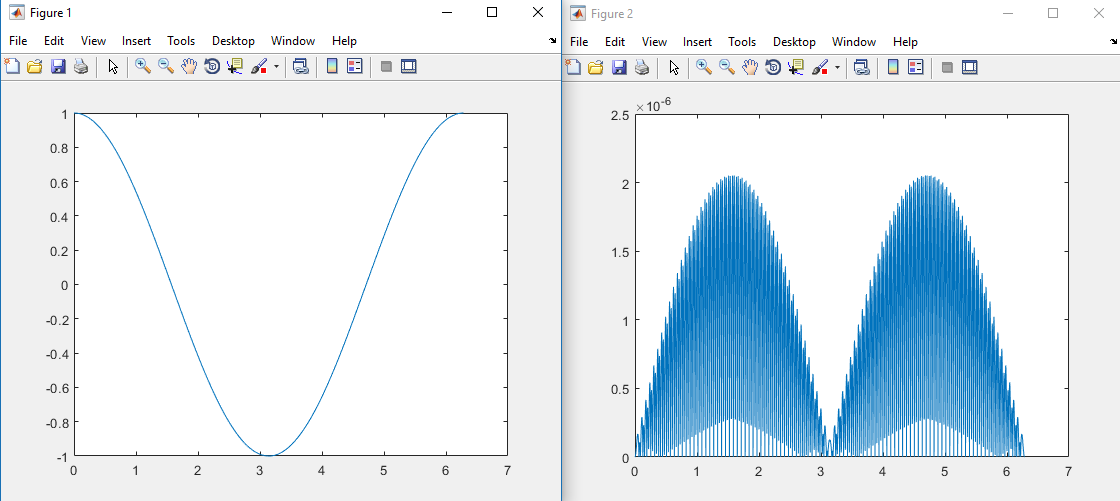
\includegraphics[scale=0.55]{hw2g1}
		\end{center} 
	
	\end{enumerate}
	
	
\end{document}